\chapter{Tau Lifetime Studies}

\section{Motivation}

One of the most significant challenges faced in searches for heavy resonances decaying to tau pairs is the presence of neutrinos in the tau decays. Hadronic tau decays produce one neutrino, and leptonic tau decays produce two neutrinos so that, depending on the channel studied, each di-tau event may have two, three, or four neutrinos present in the decay products. These neutrinos do not interact with the detector, and carry energy away from the event. Information about the neutrinos can only be inferred from $\MET$, an event-level (as opposed to particle-level) quantity which estimates the net (event-wide) neutrino momentum in the transverse direction. If, for example, two neutrinos are produced back-to-back, the only recoverable information about them is the net difference in transverse momentum. Given that the taus, and by extension their decay products, are generated back-to-back in $Z^\prime$ decays, $\MET$ alone does not provide sufficient information to precisely model the di-tau mass. The current mass estimator used in the 8 TeV and 13 TeV $Z^\prime\to\tau\tau$ searches, $\massvis$, depends on $\MET$ and, as shown in Figure \ref{fig:massVisSigVsMC}, suffers due to this loss of information.

\begin{figure}[tbh!]
\centering
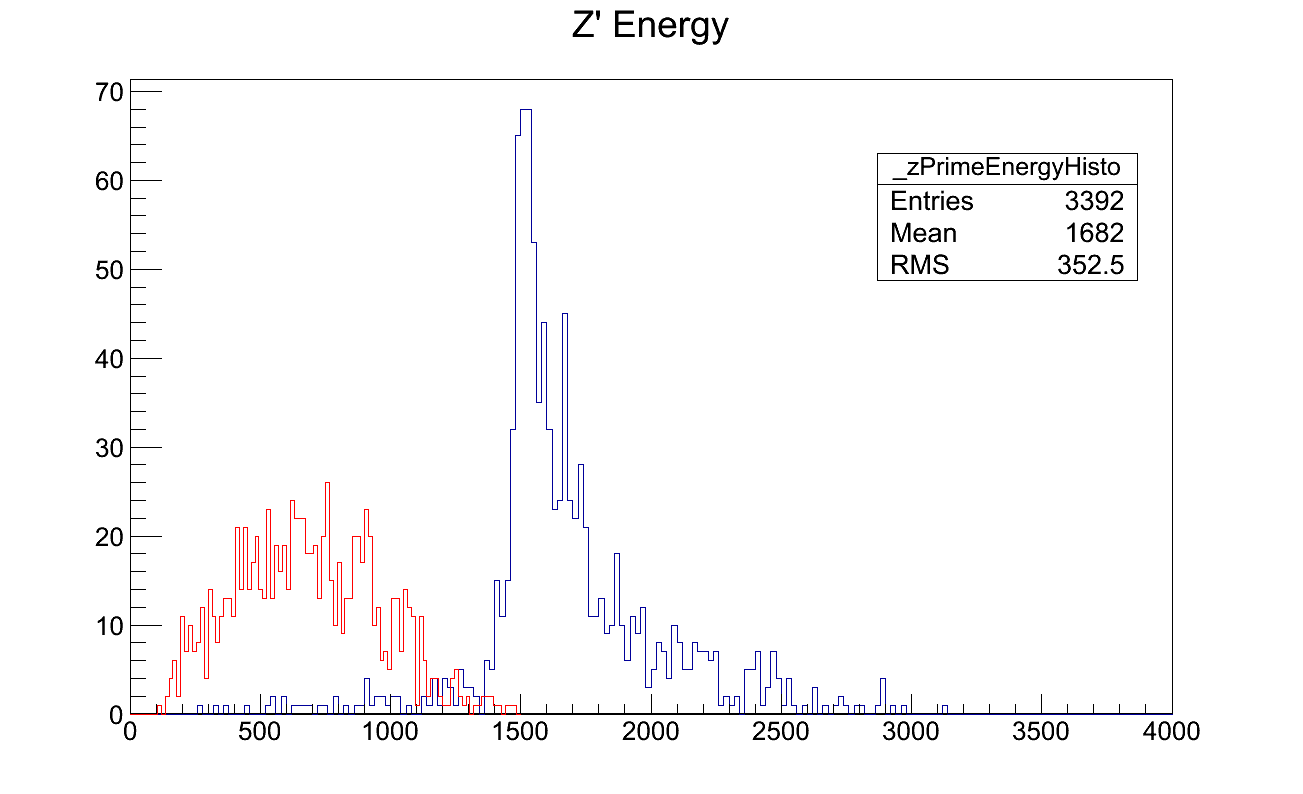
\includegraphics[width=0.6\textwidth]{figures/ZPrime1500EnergyMassVisOverlay.png}
\caption{1.5 TeV $Z^\prime$ generated energy (blue) compared to reconstructed visible mass, $\massvis$ (red). The $\massvis$ distribution is broader and peaked at a much lower energy than the MC truth.}
\label{fig:massVisSigVsMC}
\end{figure}

One proposal to improve the discriminating power of these searches is to add additional selection criteria taking advantage of the lifetime of the tau. At $2.9\times 10^{-13}$s, the tau lifetime is quite short, but it is still long enough to distinguish decay products originating from the primary vertex from those originating from the tau decay vertex. Essentially, ``prompt" particles coming directly from the interaction point (PV) leave tracks that may be traced back to the PV, while tracks from particles coming from tau decays will ``miss" the PV due to the distance the tau traveled from the PV before decaying. This concept is illustrated in Figure \ref{fig:PromptVsTauDecay}. These additional selection critera, referred to as ``lifetime cuts," are based on tracking information collected from the tau decay products.

\begin{figure}[tbh!]
\centering
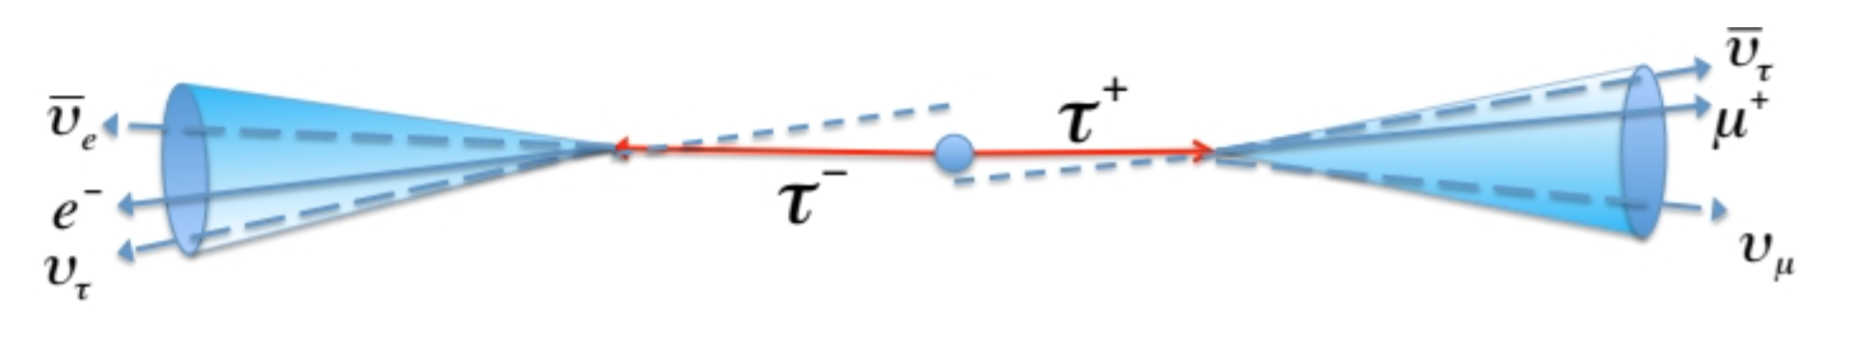
\includegraphics[width=1.0\textwidth]{figures/DiTauDecay.png}
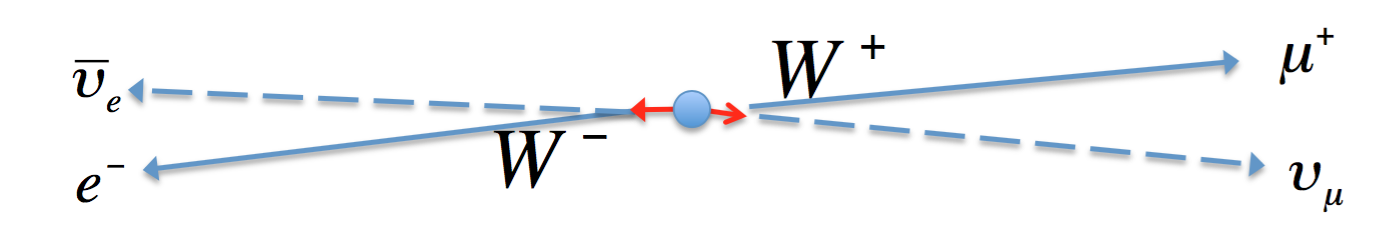
\includegraphics[width=1.0\textwidth]{figures/WWDecay.png}
\caption{A ditau event (top) will produce decay products whose tracks miss the PV, whereas leptonic decays from a shorter-lived parent produced in the $pp$ collision, such as a $W^+W_-$ event (bottom), will produce ``prompt" leptons which can be traced back to the PV.}
\label{fig:PromptVsTauDecay}
\end{figure}

\section{Methods}

Efforts to study the efficacy of the tau lifetime cuts began in the $\emu$ channel with a simple cut on the individual impact parameters of the electron and muon in each ditau event. In this channel, the principal prompt backgrounds are $t\bar{t}$, where the $b$ quarks from $t$ decays decay leptonically into an electron and muon, and $W^+W_-$, where the $W$s decay leptonically into an electron and muon. Drell-Yan events where virtual $Z$ bosons decay into tau pairs are in principle an irreducible background, but the rate falls off significantly in the high-mass (signal) region being considered.

The cut was first defined as the sum of the absolute values of the impact parameters (IPs) of each lepton:

\begin{equation}
\centering
\nomath{Lifetime}_\tau = |\nomath{IP}_e| + |\nomath{IP}_\mu|

\end{equation}

\noindent To account for the large variance in track resolution, and thus prefentially-select ``clean" tau decays, the lifetime definition was modified to include the track measurement error:

\begin{equation}
\centering
\nomath{Lifetime}_\tau = \sqrt{\frac{\left(|\nomath{IP}_e| + |\nomath{IP}_\mu|\right)^2}{\sigma_{\nomath{IP}_e}^2 + \sigma_{\nomath{IP}_\mu}^2}}

\label{eq:IP}

\end{equation}

The cut is placed at the very end of the selection sequence, immediately following the b-jet veto. The quantity in Equation \ref{eq:IP} is required to exceed a value chosen based on optimization studies. These studies, based in signal and background MC, compare the acceptance of signal events with the rejection of background events across several values of this threshold. The threshold value is chosen based on its associated value of $\frac{s}{\sqrt{s+b}$, where $s$ is the signal rate and $b$ is the aggregated background rate. Figure \ref{fig:IPstudy} shows the performance of the impact-parameter-based lifetime cut in MC. A cut threshold of 2 was chosen on the basis of maximizing both $\frac{s}{\sqrt{s+b}$ and signal MC acceptance.


\begin{figure}[tbh!]
\centering
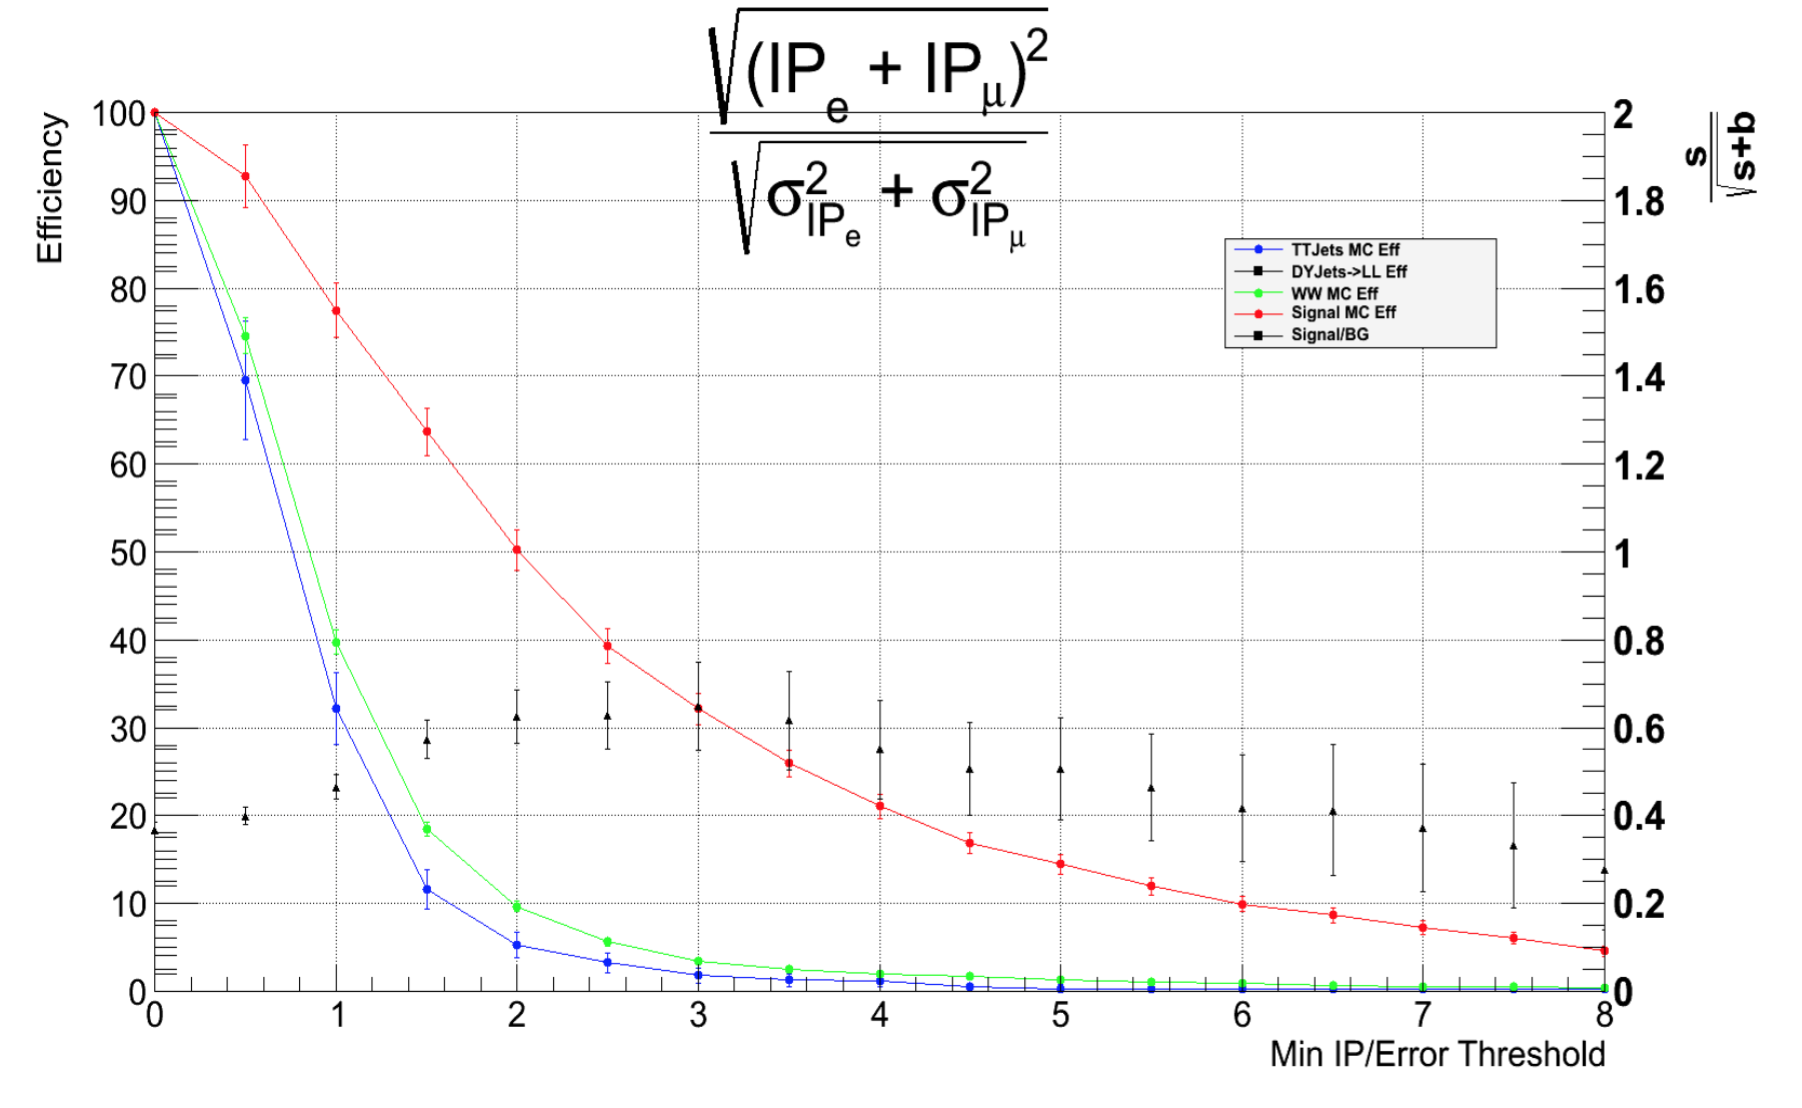
\includegraphics[width=1.0\textwidth]{figures/IPstudy.png}
\caption{Plot showing the performance of the impact-parameter definition of the lifetime cut. The colored lines indicate MC efficiencies and correspond to the left axis. The black triangles indicate $\frac{s}{\sqrt{s+b}$ and correspond to the right axis. A threshold value of 2 was chosen for the cut since it is the first value on the plateau of $\frac{s}{\sqrt{s+b}$ maxima, thereby keeping signal MC acceptance as high as possible.}
\label{fig:IPstudy}
\end{figure}
